\documentclass[review]{elsarticle}

\usepackage{lineno,hyperref}
\modulolinenumbers[5]

\journal{To Discuss With FIT Collaboration}

%%%%%%%%%%%%%%%%%%%%%%%
%% Elsevier bibliography styles
%%%%%%%%%%%%%%%%%%%%%%%
%% To change the style, put a % in front of the second line of the current style and
%% remove the % from the second line of the style you would like to use.
%%%%%%%%%%%%%%%%%%%%%%%

%% Numbered
%\bibliographystyle{model1-num-names}

%% Numbered without titles
%\bibliographystyle{model1a-num-names}

%% Harvard
%\bibliographystyle{model2-names.bst}\biboptions{authoryear}

%% Vancouver numbered
%\usepackage{numcompress}\bibliographystyle{model3-num-names}

%% Vancouver name/year
%\usepackage{numcompress}\bibliographystyle{model4-names}\biboptions{authoryear}

%% APA style
%\bibliographystyle{model5-names}\biboptions{authoryear}

%% AMA style
%\usepackage{numcompress}\bibliographystyle{model6-num-names}

%% `Elsevier LaTeX' style
\bibliographystyle{elsarticle-num}
%%%%%%%%%%%%%%%%%%%%%%%

\begin{document}

\begin{frontmatter}

\title{Analysis Of Fuel Loading Management in Fuel Cycle Simulation Tools In The Framework Of The FIT Project}
%\tnotetext[mytitlenote]{Fully documented templates are available in the elsarticle package on \href{http://www.ctan.org/tex-archive/macros/latex/contrib/elsarticle}{CTAN}.}

%% Group authors per affiliation. 
% Rules for Author List : Two groups 
% Group 1 = Main contributors (calculations and/or significative helping writing)
% Group 2 = Other membre of the FIT Project
% Main writer is Corresponding Autor

% Group 1

\author[IPNO]{X.~Doligez}
\author[ANL]{B.~Feng}
\author[BUD]{M.~Halasz}
\author[SCK]{A.~Hernandez}
\author[MAULE]{I.~Merino}
\author[MAD]{B.~Mouginot}
\author[CIEMAT]{A.V.~Skarbeli}

\author[SUB]{N. Thiolli\`ere \corref{cor1}}
\ead{nicolas.thiolliere@subatech.in2p3.fr}

% Group 2
\author[CIEMAT]{F.~Alvarez-Velarde}
\author[ORNL]{E.~E.~Davidson}
\author[TRACT]{H.~Druenne}
\author[IPNO]{M.~Ernoult}
\author[USC]{R.~Flanagan}
\author[INL]{R.~Hays}
\author[SCK]{A.~Hernandez}
\author[UI]{K.~Huff}
\author[BUD]{M.~Szieberth}
\author[TRACT]{B.~Vermeeren}
\author[CIEMAT]{A.~Villacorta}
\author[MAD]{P.~Wilson}

\cortext[cor1]{Corresponding author}

\address[IPNO]{Institut de Physique Nucléaire d’Orsay, CNRS-IN2P3/Univ, Paris-Sud, France}
\address[ANL]{Argonne National Laboratory, 9700 Cass Ave., Lemont, IL 60439, USA}
\address[BUD]{Budapest University of Technology and Economics (BME), Institute of Nuclear Techniques, 1111 Budapest, Müegyetem rkp. 3-9, Hungary}
\address[SCK]{Studiecentrum voor kernenergie - Centre d'étude de l'énergie nucléaire (SCK-CEN), Boeretang 200, Mol, Belgium}
\address[MAULE]{Catholic University of the Maule, Av. San Miguel 3605, Talca, Chile}
\address[MAD]{Univ. of Wisconsin Madison, Department of Nuclear Engineering and Engineering Physics, Madison, WI, United States}
\address[SUB]{Subatech, IMTA-IN2P3/CNRS-Universit\'e, Nantes, F-44307, France}
\address[ORNL]{Oak Ridge National Laboratory, Building 5700, Mail Stop 6172, Oak Ridge, TN 37831, United States}
\address[TRACT]{Tractebel Engie, Boulevard Simón Bolívar 34-36, 1000 Brussels, Belgium}
\address[USC]{University of South Carolina, Nuclear Engineering Program, Columbia, SC 29201, United States}
\address[INL]{Idaho National Laboratory, 2525 Fremont Ave., Idaho Falls, ID 83402, USA}
\address[UI]{University of Illinois, Department of Nuclear, Plasma, and Radiological Engineering, United States}
\address[CIEMAT]{CIEMAT, Avda. Complutense, 40, 28040 Madrid, Spain}

\begin{abstract}
Abstract beginning...


In this paper, the first tested functionality is presented. The impact of the fuel composition dependency with stock versus a fixed fraction approach is tested. Results from different methodologies are compared.
\end{abstract}

\begin{keyword}
Nuclear Fuel Cycle \sep Simulation \sep Functionality \sep Benchmark
\end{keyword}

\end{frontmatter}

\linenumbers

% #########################################################################################
% #########################################################################################
% #########################################################################################
\section{Introduction}

Since the 1990’s, many different fuel cycle systems tools have been developed by several institutions (industrial, engineering, academic, etc.). These tools vary in terms complexity, from a simple spreadsheet model to a complex simulation code framework. These tools have evolved and new tools have been developed to leverage the constantly increasing computational power availability. Many of these tools can be used at different levels of detail and can be adapted for specific problem or any problem related to the nuclear fuel cycle.

The fuel cycle systems tools of interest in this activity are dynamic fuel cycle simulators. They are an essential part of the technical evaluation of the future deployment of innovative nuclear systems. Also, they help identify drivers and interactions between parameters in fuel cycle fleet physics. Finally, these tools produce data for further assessments (economy, safety, non-proliferation, etc.) that can be internal or external to the tool. For these reasons, fuel cycle simulators can be viewed as vital tools to inform and support decisions related to the nuclear fuel cycle of a country or multiple countries.

Many of these tools were developed independently by a single institution and oftentimes by a single individual with limited feedback from an established user community or from other developers. There have been multiple international fuel cycle code benchmarks in the past but these were dedicated to comparing detailed time-dependent results for fully-described fuel cycle system evolution over time with limited comparisons of specific tool functionality. The goal of this project is to also improve the confidence in the calculations of these fuel cycle simulators, but with more of a focus on comparing different tool functionality in isolation, hence the name Functionality Isolation Tests (FIT). The purpose of the project is to test the impact of a Fuel Cycle Code (FCC) functionality and how this impact is propagated over time in the fully-described fuel cycle system calculations.

% #########################################################################################
% #########################################################################################
% #########################################################################################
\section{Description Of The FIT Project}
\subsection{Glossary and definitions}
\subsubsection{Reactor Physics Code (RPC)}

A Reactor Physics Code is used to simulate the neutron behavior in a unit cell, a fuel assembly or a nuclear core. It can be deterministic or stochastic and is also plugged with a Bateman Solver for solving evolution (a.k.a. burnup/depletion) equations. The input is the description of the system and the initial fuel composition. The output is the evolution of the isotopic composition or other data, such as reactivity or mean cross sections. 

\subsubsection{Fuel Cycle Code (FCC)}

A Fuel Cycle Code is a dynamic fuel cycle simulation tool. The aim is to model an evolving electro-nuclear fleet. The main output is the evolution of isotopes everywhere in all facilities.

\subsubsection{Fuel Loading Model (FLM)}

A FLM aims to adapt the fresh fuel composition according to the reactor requirements. For instance, the fissile fraction is calculated from the fissile stock quality in order to reach the required burnup of the reactor. A FLM could be based on neural network, Plutonium equivalence model, correlations, built-in depletion, etc. This relation is usually built from physics constraints and reactor physics calculations. It is possible to increase the complexity of the FLM according to the level of physics constraints. Here, FLM means there is a process that connects the fresh fuel composition to the available materials, whatever the complexity.

\subsubsection{Recipe}

A recipe approach aims to tune the fuel cycle calculation in order to have a well-known isotopic vector already precisely calculated from an external RPC. The fresh fuel composition in the reactor at Beginning Of Cycle (BOC) is always the same. For instance, the reactor loads a MOX fuel with 7\% (mass) of plutonium with always the same isotopic composition. It is possible to use recipe interpolation, closest composition, etc.  

\subsubsection{Fixed Fraction}

We call Fixed Fraction approach a fuel cycle calculation for which each fresh fuel loading is based on the same constant fissile fraction, regardless of the isotopic vector of the fissile material. For instance, a PWR MOX is always loading a fresh fuel at 7\% of plutonium regardless of whether the Pu is 50\% Pu 239 or 95\% Pu-239. This approach is of course a major approximation for recycled fuels.

\subsection{Goals of the project}

A lot of FCC with a wide range of application. 

Dynamic Fuel Cycle Tools overview

From Simple spreadsheet to batch following tool (COSI)

FCC validation is not really possible

FCC benchmarks are complex and usually based on several level of aggregation. 

FCC benchmarks are then complex to analyse and conclusions are not clear

FCC aims to be able to reflect reality as carefully as possible

Fuel Cycle Tool is so complex (from neutron transport to nuclear fleet), simplifications are required

Compromise between complexity of functionality and induced precision improvement

FIT aims to focus on one specific functionality and to compare several models results trying to answer to one specific question. 

Methodology is kept open for all participants

The more model there is, the more information we have.

One specific exercice is solved by teams and two effects are observed:

If models provide similar/comparable results with same conclusion

What is the impact of the functionality 

\subsection{List of functionnality to test}

FLM vs constant fuel is This work

Fuel Shortage Response

Load Following VS constant load factor

Accurate physics of mixed core VS constant core

ETC.

\subsection{FIT Project involved Models}


CLASS

CYCLUS

DYMOND

ORION

VISION

Tr\_Evol / Evol\_code

ANICCA

JOSSETTE

% #########################################################################################
% #########################################################################################
% #########################################################################################
\section{Fuel Loading Model (FLM) Functionality}

In this part, the FCC functionality that updates the fuel composition is assessed by comparison with a FF approach. Specifications details are intentionally low in order to allow a high degree of freedom in the solutions for each participant. 

\subsection{Exercise specifications}

\subsubsection{Simulation requirements}

For this test, a reference calculation based on a FLM is required. That supposes to use a physics relation between fissile fraction and reactor technical requirement, such as burnup. A comparison between FLM and FF approach will be done so the possibility to bypass the FLM to use a FF is required in the fuel cycle code. For this, the fissile fraction is provided by the user. 

An optional component is to also use a reactor physics code outside of the fuel cycle code to perform the same calculation as the FLM with a fuel cycle code. This way there could be up to 3 different “solutions” for comparison purposes.

\subsubsection{Reactor design and fuel}

Given the different tools, methods, and specialization of each institution, it will not be possible for every institution to model the same reactor exactly the same way and fairly compare results across different codes (this would be a code-to-code comparison, which is not the purpose of the FIT Benchmarks). This is why we will allow each participant to model the specific reactor/fuel design(s) with which they are more familiar and for which they may already have models, as long as they fit the general guideline (specification) that one of these models is for a fast spectrum (e.g., metallic fuel in SFR) and another one is for a thermal spectrum (e.g., MOX fuel in PWR).

\subsubsection{Facilities}

For this exercise, the following facilities may be required: 

\begin{itemize}
    \item A fissile stock with a plutonium vector (enough to operate one cycle)
    \item A fertile stock with a depleted uranium vector
    \item A fabrication plant
    \item A reactor
    \item A storage for the spent fuel
\end{itemize}

A schematic representation of the fuel cycle is proposed on the Figure~\ref{fig:Scenario}

\begin{figure}
    \centering
    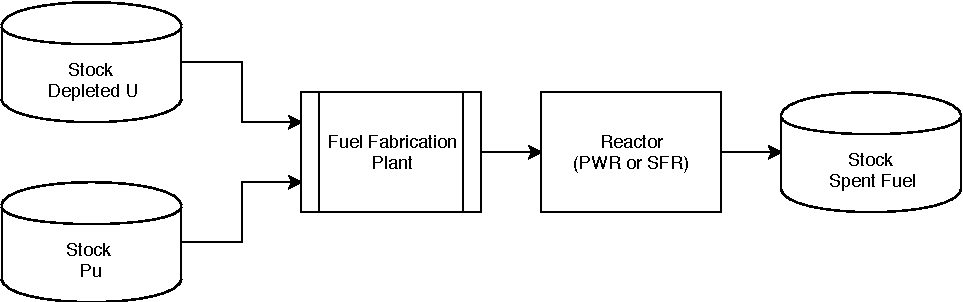
\includegraphics[width=0.99\textwidth]{FIG/FuelCycleDiagram.pdf}
    \caption{Schematic representation of the fuel cycle used for the exercise.}
    \label{fig:Scenario}
\end{figure}

\subsubsection{Time frame}

The simulation has to be run on a full reactor cycle duration. The relation between the fuel cycle time $Dt$, the reactor power $P_{th}$, heavy nuclide mass $M$ and the burn-up $BU$ is then given by : 

\begin{equation}
BU = \frac{P_{Th} \cdot Dt}{M}
\end{equation}

At t = 0, the fresh fuel is built inside the fabrication plant according to reactor requirements. The fabrication time is zero and the reactor is loaded instantaneously. A complete fuel cycle is run and the spent fuel is sent to stock when the required BU is reached.

\subsubsection{Plutonium vector}

The plutonium vectors that will be tested in the framework of this exercise needs to be representative of realistic case. The Table~\ref{tab:PuVector} shows minimum and maximum isotopic fraction and total fraction in the fuel. 

\begin{table}[]
\begin{center}
    \begin{tabular}{|l|l|l|}
        \hline
        Isotope & Min. fraction (wgt \%) & Max. fraction (wgt \%) \\
        \hline
        Pu @BOC in fuel (PWR) & 5 & 10 \\
        Pu @BOC in fuel (SFR) & 13 & 22 \\
        \hline
        $^{238}$Pu & 0 & 10 \\
        $^{239}$Pu & 25 & 90 \\
        $^{240}$Pu & 10 & 40 \\
        $^{241}$Pu & 0 & 25 \\
        $^{242}$Pu & 0 & 30 \\
        $^{241}$Am & 0 & 10 \\
        \hline
    \end{tabular}
\end{center}
\caption{Plutonium vector characteristics at Beginning Of Cycle (BOC) in PWR or SFR reactors. Plutonium weight fraction is provided in weight \% as a fraction of heavy mass in the fuel. Isotopic fraction represents weight fraction in the plutonium vector.}
\label{tab:PuVector}
\end{table}


Each user can use a different plutonium vector as long as it is included inside this range.
    
\subsubsection{Methodology}

Each participant of the project defines its own methodology according to the specificity of the FCC used. The only constraint is to define a method that produces a comparison between the reference calculation based either on FCC/FLM or Recipe approach and the FF approach. Methodology defined in the framework of this exercise will be detailed on part~\ref{section:Methodology}.

\subsection{Methodology description}\label{section:Methodology}




    \subsubsection{Sampling method}

CLASS, CYCLUS and JOSSETTE

    \subsubsection{Method from ANICCA}

SEE DOC

    \subsubsection{Method from CIEMAT}

SEE DOC

    \subsubsection{Method from Teddy}

Think What to do...

    \subsubsection{Method from Bo Feng}

Think what to do...







% #########################################################################################
% #########################################################################################
% #########################################################################################
\section*{References}

\bibliography{mybibfile}

\end{document}
